
\documentclass[10pt, twoside, openright, a5paper]{report}
\let\openright=\cleardoublepage

\usepackage[a-2u]{pdfx}

\usepackage{fontspec}
\setmainfont{Libertinus Serif}
\setsansfont{Libertinus Sans}
\newfontfamily\figfamily{Libertinus Serif}
\setmonofont{IBM Plex Mono Light}[BoldFont={IBM Plex Mono Semibold}, Ligatures=CommonOff,Scale=0.86]


\usepackage[textwidth=4.5in]{geometry}

\usepackage{amsmath,amsfonts,amsthm}
\usepackage{unicode-math}
\usepackage{pdfpages}
\usepackage{graphicx}
\usepackage{marginnote}
\usepackage{ifoddpage}
\usepackage[all]{nowidow}
\usepackage[shortlabels]{enumitem}

\usepackage{listings}

\usepackage{algpseudocode}
\usepackage{algorithm}
\usepackage{caption}
\DeclareCaptionFont{fig}{\figfamily}
\captionsetup{font={footnotesize,fig},labelfont=bf,labelsep=quad}
\DeclareCaptionStyle{ruled}{font={footnotesize,fig},labelfont=bf,labelsep=quad,strut=off}

\usepackage{chngcntr}
\counterwithout{figure}{chapter}
\counterwithout{table}{chapter}

\usepackage[natbib,style=ext-numeric-comp,sorting=none,articlein=false,maxnames=6,maxcitenames=1]{biblatex}

\addbibresource{bibliography.bib}
\addbibresource{myrefs.bib}
%\DeclareNameAlias{sortname}{family-given}
%\DeclareNameAlias{default}{family-given}
\DeclareFieldFormat*{volume}{\mkbibbold{#1}}
\DeclareDelimFormat{namelabeldelim}{~}
\renewcommand*{\bibfont}{\scriptsize}

\usepackage{booktabs}
\usepackage{xcolor}

\usepackage{tikz}
\usetikzlibrary{shapes,decorations.markings,positioning,calc,arrows.meta,matrix,fit,decorations.pathreplacing}
\pgfdeclarelayer{background}
\pgfsetlayers{background,main}

\usepackage{chemfig}

\usepackage{minted}
\usemintedstyle{vs}
\colorlet{LightGray}{black!3}
\newmintedfile[inputmintedcpp]{c++}{bgcolor=LightGray,tabsize=2,fontsize=\scriptsize,linenos,breaklines,escapeinside=\#\#}
\def\FancyVerbVspace{0pt}
\AtBeginEnvironment{minted@colorbg}{\setlength{\medskipamount}{0pt}}

\usepackage{subcaption}

\newcommand{\xxx}[1]{\textcolor{red}{#1}}

% Thesis title in English (exactly as in the formal assignment)
\def\ThesisTitle{Employing Parallel Computing in Data-Intensive Tasks}

% Author of the thesis
\def\ThesisAuthor{Adam Šmelko}

% Year when the thesis is submitted
\def\YearSubmitted{2024}

% Name of the department or institute, where the work was officially assigned
% (according to the Organizational Structure of MFF UK in English,
% or a full name of a department outside MFF)
\def\Department{Department of Distributed and Dependable Systems}

% Is it a department (katedra), or an institute (ústav)?
\def\DeptType{Department}

% Thesis supervisor: name, surname and titles
\def\Supervisor{Martin Kruliš}

% Supervisor's department (again according to Organizational structure of MFF)
\def\SupervisorsDepartment{Department of Distributed and Dependable Systems}

% Study programme and specialization
\def\StudyProgramme{Computer Science --- Software Systems}

% An optional dedication: you can thank whomever you wish (your supervisor,
% consultant, a person who lent the software, etc.)
\def\Dedication{%
I dedicate this thesis to my family, friends, and colleagues who have supported me throughout my studies.

I thank colleagues from Department of Bioinformatics, Department of Physics of Materials, LCSB, BSC, Institut Curie, and especially colleagues from my department for great challenges and research opportunities they have brought. I extend my gratitude to my closest friends for their support, vivid discussions over drinks and food, and for keeping my (in)sanity at bay. I thank Nikola, who has always been there for me, and my family for their unconditional love and support.

Most importantly, I would like to thank my supervisor, Martin Kruliš, for his guidance, patience, and valuable feedback. His professional mentorship has been invaluable to me, and I am grateful for the opportunity to work with him.
}

% Abstract (recommended length around 80-200 words; this is not a copy of your thesis assignment!)
\def\Abstract{%
This thesis studies, develops, and investigates the optimization of data-intensive scientific algorithms using Graphics Processing Units (GPUs) to enhance performance and scalability. The first part of the thesis focuses on the design and implementation of optimized kernels for four key algorithms: hierarchical clustering with Mahalanobis linkage, neighborhood-based dimensionality reduction through EmbedSOM, optimization of cross-correlation algorithms for many small inputs, and stochastic simulation of Boolean networks. In the second part, the thesis builds upon the findings of the first part to propose a Noarr library, which enables the efficient development of high-performance computing (HPC) applications. It emphasizes the critical role of memory optimization in achieving significant performance improvements in HPC and aims to streamline the implementation of these optimizations by providing a novel memory layout and traversal optimization framework. The main contributions of this thesis comprise the implementation of novel GPU optimization techniques, performance improvements of scientific tools of up to three orders of magnitude speedup, advancing data analysis and visualization in bioinformatics and material physics, and the design of new tools for efficient expression of data structure layout and traversal in HPC code. The results of this thesis may be used to enhance the development process of maintainable and efficient HPC applications and guide future research in the field of data-intensive scientific computing.
}

% 3 to 5 keywords (recommended), each enclosed in curly braces
\def\Keywords{%
{GPGPU}, {HPC}, {hierarchical clustering}, {cross-correlation}, {memory optimizations}, {loop transformations}
}

\hypersetup{unicode}
\hypersetup{breaklinks=true}
\hypersetup{hidelinks}

\usepackage[capitalize]{cleveref}

%%% This file contains definitions of various useful macros and environments %%%
%%% Please add more macros here instead of cluttering other files with them. %%%

%%% Minor tweaks of style

% This macro defines a chapter, which is not numbered, but is included
% in the table of contents.
\def\chapwithtoc#1{
\chapter*{#1}
\addcontentsline{toc}{chapter}{#1}
}

\def\secwithtoc#1{
\section*{#1}
\addcontentsline{toc}{section}{#1}
}

% Draw black "slugs" whenever a line overflows, so that we can spot it easily.
\overfullrule=5mm
\emergencystretch=1cm

\AtBeginDocument{
\hyphenation{SOM-Hun-ter}
\hyphenation{Wi-de-spread}
}

%%% Macros for definitions, theorems, claims, examples, ... (requires amsthm package)

\theoremstyle{plain}
\newtheorem{thm}{Theorem}
\newtheorem{lemma}[thm]{Lemma}
\newtheorem{claim}[thm]{Claim}

\theoremstyle{plain}
\newtheorem{defn}{Definition}
\newtheorem{problem}{Problem}

\theoremstyle{remark}
\newtheorem*{cor}{Corollary}
\newtheorem*{rem}{Remark}

%%% An environment for proofs

\newenvironment{myproof}{
  \par\medskip\noindent
  \textit{Proof}.
}{
\newline
\rightline{$\qedsymbol$}
}

%%% The field of all real and natural numbers
\newcommand{\R}{\mathbb{R}}
\newcommand{\N}{\mathbb{N}}
\newcommand{\Asymp}[1]{\ensuremath{\mathcal{O}\left(#1\right)}}

%%% Useful operators for statistics and probability
\DeclareMathOperator{\pr}{\textsf{P}}
\DeclareMathOperator{\E}{\textsf{E}\,}
\DeclareMathOperator{\var}{\textrm{var}}
\DeclareMathOperator{\sd}{\textrm{sd}}
\DeclareMathOperator{\subs}{\textsc{Sub}}

% contributions
\newcounter{contribution}
\def\contribution#1{
\refstepcounter{contribution}
\chapter*{Contribution \arabic{contribution}\\#1}
\addcontentsline{toc}{chapter}{Contribution \arabic{contribution}\\#1}
}

\crefname{contribution}{contribution}{contributions}
\Crefname{contribution}{Contribution}{Contributions}

\setlength{\marginparpush}{0pt}
\setlength{\marginparsep}{2em}

\newcommand{\contribmark}[1]{%
\hyperref[#1]{\begin{tikzpicture}[ultra thick, font=\sf\bfseries]
\node[regular polygon, regular polygon sides=3, rounded corners=0.3ex, inner sep=.3ex,draw] (ll) {\ref*{#1}};
\end{tikzpicture}}}
\newcommand{\margincontrib}[1]{\marginnote{\contribmark{#1}}}

\newcommand{\publishedas}[1]{\begin{description}\item[Published as]\begin{refsection}\fullcite{#1}\end{refsection}\end{description}}

% ONLINE VERSION without the manuscripts
\newif\ifonlineversion
\onlineversiontrue
%\onlineversionfalse
\newcommand\onlineomit[1]{\ifonlineversion\vfill\begin{center}\fbox{\parbox{16.5em}{\footnotesize A re-printed manuscript that would appear here is omitted in the electronic version of the thesis.}}\end{center}\vfill\else#1\fi}

% publication contributions
\def\contF{
\begin{tikzpicture}\fill circle(0.666ex);\end{tikzpicture}}
\def\contP{
\begin{tikzpicture}\begin{scope}[rotate=90]\clip circle(0.666ex);\fill (-0.666ex,-0.666ex) rectangle(-0.1ex,0.666ex);\end{scope}\draw circle(0.666ex);\end{tikzpicture}}
\def\contN{\begin{tikzpicture}\draw[densely dotted] circle(0.666ex);\end{tikzpicture}}

% chemfig style
\renewcommand*\printatom[1]{\ensuremath{\mathsf{#1}}}
\setchemfig{atom sep=4ex, angle increment=30}
\catcode`\_=11
\tikzset{
	ddbond/.style args={#1}{
		draw=none,
		decoration={%
			markings,
			mark=at position 0 with {
				\coordinate (CF@startdeloc) at (0,\dimexpr#1\CF_doublesep/2)
				coordinate (CF@startaxis) at (0,\dimexpr-#1\CF_doublesep/2);
			},
			mark=at position 1 with {
				\coordinate (CF@enddeloc) at (0,\dimexpr#1\CF_doublesep/2)
				coordinate (CF@endaxis) at (0,\dimexpr-#1\CF_doublesep/2);
				\draw[dash pattern=on 2pt off 1.5pt] (CF@startdeloc)--(CF@enddeloc);
				\draw (CF@startaxis)--(CF@endaxis);
			}
		},
		postaction={decorate}
	}
}
\catcode`\_=8

% latexdiff preamble commands:
%DIF UNDERLINE PREAMBLE %DIF PREAMBLE
\RequirePackage[normalem]{ulem} %DIF PREAMBLE
\RequirePackage{color}\definecolor{RED}{rgb}{1,0,0}\definecolor{BLUE}{rgb}{0,0,1} %DIF PREAMBLE
\providecommand{\DIFadd}[1]{{\protect\color{green!50!black}\uwave{#1}}} %DIF PREAMBLE
\providecommand{\DIFdel}[1]{{\protect\color{red}\sout{#1}}}                      %DIF PREAMBLE
%DIF SAFE PREAMBLE %DIF PREAMBLE
\providecommand{\DIFaddbegin}{} %DIF PREAMBLE
\providecommand{\DIFaddend}{} %DIF PREAMBLE
\providecommand{\DIFdelbegin}{} %DIF PREAMBLE
\providecommand{\DIFdelend}{} %DIF PREAMBLE
\providecommand{\DIFmodbegin}{} %DIF PREAMBLE
\providecommand{\DIFmodend}{} %DIF PREAMBLE
%DIF FLOATSAFE PREAMBLE %DIF PREAMBLE
\providecommand{\DIFaddFL}[1]{\DIFadd{#1}} %DIF PREAMBLE
\providecommand{\DIFdelFL}[1]{\DIFdel{#1}} %DIF PREAMBLE
\providecommand{\DIFaddbeginFL}{} %DIF PREAMBLE
\providecommand{\DIFaddendFL}{} %DIF PREAMBLE
\providecommand{\DIFdelbeginFL}{} %DIF PREAMBLE
\providecommand{\DIFdelendFL}{} %DIF PREAMBLE


% Mahalanobis
\DeclareMathOperator{\cov}{\textbf{cov}}
\DeclareMathOperator{\mean}{mean}
\DeclareMathOperator{\argmin}{argmin}
\usepackage{titlesec}
\titlespacing*{\chapter}{0pt}{0ex}{2ex}
\titleformat{\chapter}{\LARGE\bfseries\sloppy}{\thechapter}{1em}{}{}
\makeatletter\@openrightfalse\makeatother

\begin{document}
%%% Title page of the thesis and other mandatory pages

%%% Title page of the thesis

\pagestyle{empty}

\hypersetup{pageanchor=false}
\begin{center}

\centerline{\mbox{
\includegraphics[width=117mm]{img/logo-en.pdf}}}

\vfill

{\bfseries\Large ABSTRACT OF DOCTORAL THESIS}

\vfill

{\Large\ThesisAuthor}

\vspace{2ex}

{\Large\bfseries\ThesisTitle}

\vfill

\Department

\vfill

{
\small
\centerline{\vbox{\halign{\hbox to 0.45\hsize{\hfil #}&\hskip 0.5em\parbox[t]{0.45\hsize}{\raggedright #}\cr
Thesis supervisor:&\Supervisor \cr
Study programme:&\StudyProgramme \cr
}}}}

\vfill

% Zde doplňte rok
Prague \YearSubmitted

\end{center}

\newpage

%%% Mandatory information page of the thesis

{
\small
\setlength\parindent{0mm}
\setlength\parskip{2pt}
The results of the thesis were achieved in the period of a doctoral study at
the Faculty of Mathematics and Physics, Charles University in Prague in years
2020--2024.

\begin{center}
\begin{tabular}{rl}
Student:
 & Mgr. Adam Šmelko \\
Supervisor:
 & doc. RNDr. Martin Kruliš, Ph.D. \\
 & Department of Distributed and Dependable Systems \\
 & Faculty of Mathematics and Physics \\
 & Charles University in Prague \\
 & Malostranské náměstí 25, 11800 Prague 1 \\
\addlinespace
Department:
 & Department of Distributed and Dependable Systems \\
 & Faculty of Mathematics and Physics \\
 & Charles University in Prague \\
 & Malostranské náměstí 25, 11800 Prague 1 \\
\addlinespace
Opponents:
 & Dr. Carlos Álvarez Martínez \\
 & Department of Computer Architecture \\
 & Universitat Politècnica de Catalunya  \\
 & Carrer de Jordi Girona 1, 08034 Barcelona \\
 \addlinespace
 & doc. Ing. Jiří Jaroš, Ph.D. \\
 & Department of Computer Systems \\
 & Faculty of Information Technology \\
 & Božetěchova 1/2, 61266 Brno \\
\end{tabular}
\end{center}

The thesis defence will take place on 26th September 2024 at 14:00 a.m. in front
of a commitee for thesis defense in the branch P4I2 (Software Systems) at the
Faculty of Mathematics and Physics, Charles University in Prague, Malostranské
náměstí 25, Prague 1, attended virtually using Zoom.

\begin{center}
\begin{tabular}{rl}
Chairman of Academic Council P4I2: \hspace{-0.5em}
 & doc. RNDr. Jan Kofroň, Ph.D.\\
 & Dept. of Distributed and Dependable systems\\
 & Faculty of Mathematics and Physics\\
 & Charles University in Prague\\
 & Malostranské náměstí 25, 11800 Prague 1\\
\end{tabular}
\end{center}

The thesis can be viewed at the Study Department of Doctoral Studies of the
Faculty of Mathematics and Physics, Charles University in Prague, Ke Karlovu 3,
Prague 2.

This abstract has been distributed on 5th of September 2024.
}

\newpage

%%% Mandatory information page of the thesis

{
\small
\setlength\parindent{0mm}
\setlength\parskip{2ex}

Title:
\ThesisTitle

Author:
\ThesisAuthor

\DeptType:
\Department

Supervisor:
\Supervisor, \SupervisorsDepartment

Abstract:
\Abstract

Keywords:
\Keywords
}

\newpage


\tableofcontents

\pagestyle{plain}
\pagenumbering{arabic}
\setcounter{page}{1}
\chapwithtoc{Overview}

This thesis contributes to addressing the challenges of General-purpose GPU programming (GPGPU programming) in two interconnected topics:
Firstly, the thesis couples a set of data-intensive scientific algorithms and their GPU optimizations; each contains a detailed discussion of their concurrency opportunities, memory operation analyses, and the choice of the most suitable optimization variant. Each work employs a slightly different tool in the GPU programming toolbox, showing the suitability and impact on different problems.
In the second part of the thesis, Noarr library is introduced, which builds upon the findings and expertise gained from the results of the previous part. We identified that the primary factor of many optimizations is the order of accessing data in the memory, generally referred to as \emph{memory optimizations}.
Noarr introduces reusable memory layouting primitives and provides a way to compose and traverse them in a customizable manner. The main goal of the library is to aid in writing more expressive, maintainable, and modular HPC code.

The thesis is accordingly divided into 2 larger sections, prepended by the introductory section to GPU programming. The appendix contains the reprints of the peer-reviewed publications supporting the contributions of this thesis (not present in this summary).
\chapter{Introduction to GPU programming}
\label{chap:gpu_intro}

In this chapter, we provide an overview of the GPU hardware architecture and the CUDA programming model. We also discuss the main optimization techniques used in GPU programming, which are essential for achieving high performance on GPUs. The knowledge presented in this chapter serves as a foundation for the subsequent chapters, where we detail the GPU optimizations of scientific algorithms and describe the parallelization use-cases of the Noarr library.

\section{GPU Hardware Architecture and Programming Model}
\label{sec:gpu_arch}


The main building block of a GPU is the \emph{Streaming Multiprocessor} (SM). SM couples hundreds of compute cores, a register file, L1 cache also called \emph{shared memory}, and schedulers responsible for independent scheduling of groups of threads. There are multiple SMs in a GPU, their number highly correlating with the overall GPU cost.

The abstraction of this highly parallel architecture is based on organizing threads into hierarchical levels. The basic units of execution are \emph{threads}. These are organized into \emph{blocks}, groups of threads \emph{executed on the same SM}, sharing a register file and the shared memory. Lastly, a group of blocks that is executed independently on multiple SMs is called a \emph{grid}.

Conceptually, this programming model is based on \emph{Single Instruction, Multiple Data} (SIMD) architecture, which is a type of parallel processing where a single instruction is executed on multiple data streams. In practice, SM issues threads in groups of $32$, called \emph{warps}, which execute in \emph{lockstep} --- all performing the same instruction at once. A more accurate description of this type of processing is \emph{Single Instruction, Multiple Threads} (SIMT), which is nowadays used to describe the GPU programming model.

\section{Optimizing for GPU performance}
\label{sec:gpu_optim}

Correctly applying the rich feature set of these massively-parallel machines is not trivial, as it requires a deep understanding of the architecture and programming model. Thus, achieving optimal performance on a GPU requires careful consideration of various aspects. Let us detail the most important ones to watch for when optimizing GPU code~\cite{pratx2011gpu}.

\paragraph{Arithmetic intensity}
\label{sec:arithmetic_int}

One of the most important constants in GPU programming is \emph{ops-per-byte} ratio ---  the ratio of math and memory bandwidth, and it simply determines how many math operations per transferred byte must be executed to achieve the theoretical maximum performance. For example, NVIDIA V100 datacenter GPU reaches $\approx15$ ops-per-byte ratio. As a simple rule of thumb, a program that performs less than $60$ single-precision floating point operations per single $4$-byte load/store will be \emph{memory-bound} and a program that performs more operations will be \emph{compute-bound}. Such a property of a program is called \emph{arithmetic intensity} and is a key factor in determining the performance of a GPU kernel.

\paragraph{Memory hierarchy}
\label{sec:memory_hier}

Depending on the desired level of data sharing within the thread hierarchy, programmers can use various types of memory. On a block level, on-chip shared memory can be accessed with a magnitude lower latency and higher bandwidth than global memory. In extreme data sharing cases, threads in the same warp can use the register file as a cache with close-to-zero latency. However, the higher the proximity of the specific memory type to the compute cores, the lower capacity it carries. Contemporary GPUs encompass $64$k of $32$B registers, $100-200$ kB of shared memory, and $8-16$ GB of global memory for consumer-grade GPUs and up to $80$ GB for the highest-end datacenter-grade GPUs.

\paragraph{Memory coalescing}
\label{sec:coalescing}

Fetching data from global memory is serviced in up to $128$B wide transactions. If threads in a warp request a single byte, the GPU will fetch the whole transaction chunk, wasting the memory bandwidth on data that will never be used and negatively impacting the ops-per-byte ratio. To utilize the memory bandwidth fully, the aggregated memory accesses in a lockstep should coalesce into continuous memory locations.

\paragraph{CPU--GPU data transfers}
\label{sec:transfers}

Transferring data between CPU and GPU memory spaces can pose a significant bottleneck when developing GPU programs. Usually, the interconnect which is used to transfer data between the CPU and the GPU has a much lower bandwidth even than the GPU global memory. Therefore, it is essential to avoid redundant data transfers between the host and the device.

In true data-parallel algorithms, this is generally not a big issue because these data transfers can be overlapped with computation. Such overlapping is possible by GPU \emph{task queues}, which allow the execution of multiple programs as well as CPU--GPU memory transfers in parallel. This hardware feature is exposed by the software abstraction called \emph{streams}.

\paragraph{Thread divergence}
\label{sec:divergence}

The downside of the highly parallel SIMT architecture is the necessity to handle the divergence of execution paths in the code.
If threads in a warp take different \texttt{if}-branch or their iteration count over a \texttt{while} loop does not match, the execution of these diverging paths will be serialized such that only the threads active in \emph{the same execution path} will be executed in lockstep.

\paragraph{Thread occupancy}
\label{sec:occupancy}

A single SM can accommodate thousands of concurrent threads, although the number of accommodable cores is a magnitude lower. The SM takes advantage of this high discrepancy to aggressively context switch between different warps when the currently scheduled ones are waiting for a latency. Since all the thread contexts reside on-chip, the context switch has negligible overhead, and, provided there are enough available concurrent threads, it can effectively hide the memory latencies.

The number of concurrent threads per SM is called the \emph{thread occupancy}. This metric is influenced by the resource requirements of a program. Conversely, a GPU program that achieves high thread occupancy uses less on-chip resources, which in turn forces it to use the (slower) global memory more often, and the computational efficiency of its threads is thus lower.

\chapter[Employing GPUs in scientific algorithms]{Employing GPUs in scientific alg.}
\label{chap:gpu}


This chapter summarizes the process of porting several specific scientific algorithms to GPUs and uses these to exemplify the challenges of optimizing for GPU architectures.

\section[Mahalanobis-linkage hierarchical clustering]{Mahalanobis-linkage hierarch. clustering}
\label{sec:maha}

Hierarchical clustering is an unsupervised machine learning method that aims to group the data points into clusters according to some \emph{linkage criterion}.
In the domain of bioinformatics, hierarchical clustering with the \emph{Mahalanobis linkage} is used, which is a more sophisticated method suitable for analyzing multidimensional single-cell cytometry datasets.

Mahalanobis linkage, proposed by Fišer et al.~\cite{fivser2012detection}, allows for a very natural formation of clusters in biological data. However, the benefits come at a cost of high time and space complexity. The authors claim the upper usable bound of dataset size to be $10^4$ using the original \texttt{C} application. They state that the quadratic space complexity makes for the most significant limiting factor, leaving it unfeasible to analyze bigger datasets on current desktop computers.

\subsubsection{Algorithm complexity}

Mahalanobis linkage uses \emph{Mahalanobis distance}~\cite{mahalanobis1936generalized} to measure the similarity between clusters:
\begin{defn}[Mahalanobis distance]
    Suppose a probability distribution $C$ on $\R^d$ with mean $\bar{C} \in \R^d$ and a covariance matrix $\cov(C)$. If the matrix $\cov(C)$ is regular, we define the \emph{Mahalanobis distance} between $u \in \R^d$ and $C$ as
    \begin{equation}
    d_\text{Maha}(u,C) = \sqrt{(u-\bar{C})^T\cov(C)^{-1}(u-\bar{C})}.
    \end{equation}\label{eq01:maha}
\end{defn}

To illustrate the measure of the Mahalanobis distance, let us suppose we have two elliptic clusters. In the means of proximity, the measure favors such clusters that their ellipses are alongside rather than in a prolongation of one another~\cite{dagnelie1991using}.
Only when the objects of a cluster form a spherical shape, this dissimilarity measure is proportional to the Euclidean distance with a corresponding linkage (as depicted in Figure~\ref{fig:ellipses}).

\begin{figure}[h]
    \centering
    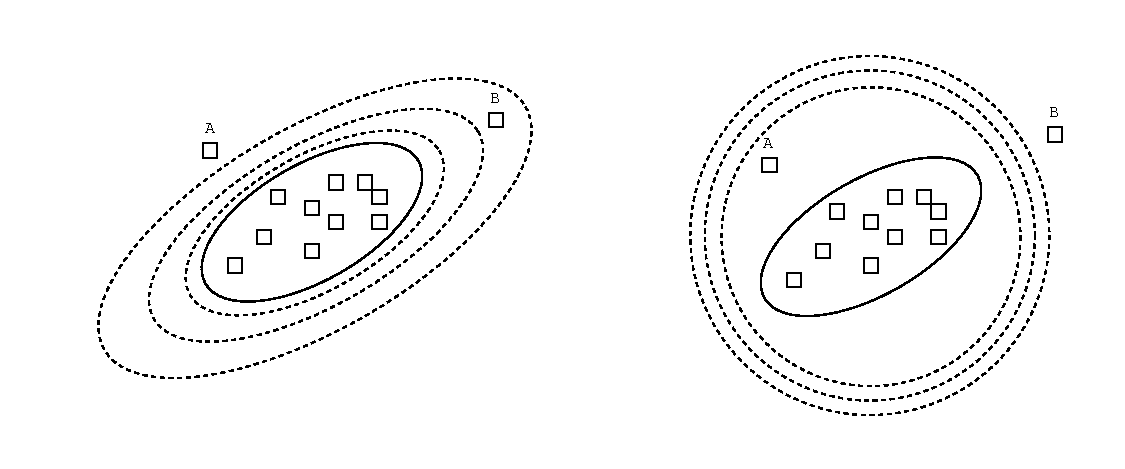
\includegraphics[width=0.8\textwidth]{img/maha.pdf}
    \caption{A comparison of the Mahalanobis (left) and Euclidean (right) distance in the context of elliptic clusters. The contour lines represent the space of the equal distance from the cluster centroid.}
    \label{fig:ellipses}
\end{figure}

The standard Hierarchical Clustering (HC), which utilizes a dissimilarity matrix, has a time complexity of $\mathcal{O}(n^3)$ and space complexity of $\mathcal{O}(n^2)$. There are other variants of HC which use a different method for the closest cluster pair retrieval and the amount of distances to recompute after each iteration. Other variants include HC with the nearest neighbor array, which trades the linear memory complexity for a worse time complexity on average, or the HC with priority queues, which reduces the time complexity to $\mathcal{O}(n^2 \log n)$ for the sake of bigger memory requirements~\cite{day1984efficient}.

\subsubsection{Implementation}

From the perspective of GPU programming, Mahalanobis HC is a challenging problem. Algorithms with high memory requirements are generally unfavorable for GPUs due to limited availability of global memory (refers to \nameref{sec:memory_hier} in \cref{sec:gpu_optim}). There has been a lot of work on overcoming this limitation, both from NVIDIA and the scientific community~\cite{zheng2016towards,kim2020batch,landaverde2014investigation}: CUDA has introduced \emph{unified memory}~\cite{site:cuda}, which allowed GPUs to work on data that exceeds GPU memory capacity by seamlessly copying data from CPU to GPU on page fault. This optimization can help only to a certain extent, as it can only scale to the size of CPU RAM and the data are usually sent through high-latency small-throughput interconnect (refers to \nameref{sec:transfers} in \cref{sec:gpu_optim}). Therefore, in our work, we experimented with other well-known HC variants that trade higher time complexity for a linear memory complexity --- \emph{HC with the nearest neighbor array}~\cite{day1984efficient}.

The other obstacle present in Mahalanobis HC is the greatly imbalanced workload. In the first iterations, the runtime is dominated by the complex Mahalanobis linkage computation over many pairs of $n$ clusters. But as the number of clusters decreases, the hot spot moves to the computation of the covariance matrix of a merged cluster. A naive implementation would thus leave the GPU significantly under-utilized, either because of small amount of parallelism in covariance matrix computation or in the similarity computation. To alleviate this issue, we designed a workload that uses CUDA \emph{streams} (refers to \nameref{sec:transfers} in \cref{sec:gpu_optim}), which enabled running these tasks in parallel. Consequently, this allowed us to keep the utilization of GPU cores high during the whole runtime of the algorithm.

\subsubsection{Results}

The optimized Mahalanobis HC achieves a speedup of over $1400\times$ compared to the original serial CPU implementation. We benchmarked the application on the real-world single-cytometry datasets. The biggest dataset which we benchmarked, the Samusik-All~\cite{flowrepo} ($841$ thousand $39$D points), was able to finish in the order of minutes compared to the order of days. Furthermore, we have packaged and distributed the application as a R package \texttt{gmhc} to fit workflows carried out by the bioinformatics community. To the best of our knowledge, the package enabled the scientists to analyze big datasets as a whole, increasing the accuracy of the analyzed data and decreasing the turnaround time of the analysis.




\section[Neighborhood-based dimensionality reduction]{Neighborhood-based dim. reduction}
\label{sec:embedsom}


Complementary to hierarchical clustering, a different approach to displaying cytometry datasets is \emph{dimensionality reduction} (also called \emph{embedding}), in which multidimensional cells are projected into a 2-dimensional plane, a picture, which shows cells arranged in groups with common properties.

The currently used dimensionality reduction tools are typically based on the principle of optimizing a low-dimensional embedding while preserving high-dimensional properties of interest. However, the most popular tools following this methodology, such as t-SNE~\cite{maaten2008visualizing}, UMAP~\cite{becht2019dimensionality} or TriMAP~\cite{amid2019trimap}, can suffer poor performance on large data due to the need to examine a nontrivial subset of $\binom{n}{2}$ relations (such as the pairwise distances) between $n$ data points~\cite{kratochvil2019generalized}. \emph{EmbedSOM} algorithm, introduced by Kratochvíl et al.~\cite{kratochvil2019generalized}, is designed to overcome this limitation. The costly parts of the previous methods can be omitted by creating a smaller model of the data obtained by \emph{self-organizing maps}. EmbedSOM uses the information of such an approximated manifold to compute the final embedding, retaining a competitive quality of the visualization.

Let us overview the EmbedSOM algorithm. It assumes a set of $n$ high-dimensional points $X \in \R^{n \times d}$ and the smaller data model: a set of $g << n$ high-dimensional landmarks $L \in \R^{g \times d}$, and a set of $g$ low-dimensional landmarks $l \in \R^{g \times 2}$. For each input point, $k < g$ nearest landmarks from $L$ are found (this problem is also known as $k$-NN) and assigned scores according to their distance. Finally, we compute the embedding such that the difference between distances from $l$ landmarks and the embedded point and $L$ landmarks and the original point is minimized. The minimization problem is reducible to a linear system of equations with two variables.

\subsubsection{Interactive opportunities of GPU implementation}

The main challenge of EmbedSOM is low \emph{arithmetic intensity} (refers to \nameref{sec:arithmetic_int} in \cref{sec:gpu_optim}). For GPUs, there are many ways to fight the arithmetic intensity of an algorithm, such as kernel fusion~\cite{wahib2014scalable}, leveraging the memory hierarchy~\cite{lee2012cuda} or by reordering data accesses~\cite{ghysels2012improving} and optimizing data transactions~\cite{lu2020optimizing}. Generally, these approaches can be distilled into two groups: \emph{Data sharing} and \emph{latency hiding} (refers to \nameref{sec:memory_hier} and \nameref{sec:occupancy} in \cref{sec:gpu_optim}).

We experimented with both approaches in our EmbedSOM implementation. Although L2 caches can partially handle data sharing, GPUs typically hardly benefit from them due to their low cache-to-core ratio~\cite{site:cuda}. Therefore, as one variant of $k$-NN part, we used \emph{shared memory}, a programmable cache, to store the data and landmarks. These were then used to compute all the possible pairwise distances before loading the next batch to maximize the arithmetic intensity. The second variant of the $k$-NN part used a modified \emph{bitonic sort} to find the top-$k$ landmarks. This approach has the hidden benefit of low per-thread resource requirements, resulting in higher maximum GPU occupancy and, consequently, better latency hiding (refers to \nameref{sec:occupancy} in \cref{sec:gpu_optim}).

The embedding part of EmbedSOM does not offer such caching opportunities, as each point has a different set of nearest landmarks. The only reuse can happen on the landmarks themselves. And since their count can be limited in some parameter configurations, we experimented with techniques that increase the memory bandwidth, such as \emph{vector load instructions}.

\subsubsection{Results}

Using the aforementioned optimizations, we increased the performance by $200-1000\times$ over the serial CPU version and $3-10\times$ over a na\"{i}ve GPU implementation. Furthermore, the achieved speedup enabled the interactive data visualization and was integrated into the graphical application \emph{BlosSOM}~\cite{molnarova2023throughput}. Thanks to the improved performance, the application can project datasets of up to a million points with a maintained frame rate above $30$ frames per second on consumer hardware. This contribution pushes the boundary of EmbedSOM into a semi-supervised dimensionality reduction domain, allowing users to effectively and intuitively visualize data with real-time feedback.


\section{Cross-correlation optimized for small inputs}
\label{sec:cross-correlation}

Leaving the realm of cytometry data analysis, we will focus on a highly data-bound problem: cross-correlation. This algorithm is a cornerstone of many scientific fields, such as image processing, seismology, material physics, and, with the advent of convolutional neural networks, machine learning.

The problem of cross-correlation performance was initially introduced to us by the physicists from the Department of Physics of Material at Charles University in Prague. They used the algorithm to analyze the diffraction pattern of metallic alloys from electron backscatter diffraction (EBSD) cameras to obtain the material \emph{deformation}. That can be used to study the material characteristics, such as elastic strain or lattice rotation.

The reference Python script provides the physicists with the computational throughput of tens of patterns per second. However, modern EBSD cameras produce data at a magnitude higher rate~\cite{bali2021zpracovani}. Nevertheless, thanks to the parallel nature of the problem, this is a perfect candidate for GPU acceleration.

\subsubsection{Implementation challenges}

The cross-correlation of functions $f, g: \mathbb{C}\rightarrow \R$ is defined as
\begin{equation}
    (f \star g)(\tau) = \sum_{i=-\infty}^{\infty} f(i) g(i+\tau).
\end{equation}
Figure~\ref{fig:cross-correlation} depicts the visual representation of the equation applied on a discrete case of two $2\times 2$ matrices. The matrices are shifted to produce all the possible overlaps (Figure~\ref{fig:cross-correlation}, right). For a single shift, only overlapping elements contribute to the computation: overlapped pairs are multiplied and summed together into a single output matrix element (Figure~\ref{fig:cross-correlation}, left).

\begin{figure}
    \centering
    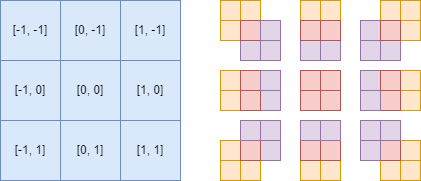
\includegraphics[width=0.6\textwidth]{img/cc.png}
    \caption{Visual representation of the cross-correlation. Yellow and purple matrices correspond to the input matrices, and the blue matrix depicts the cross-correlation output. The coordinates on the blue matrix correspond to the shift of the yellow matrix, which is depicted on the right. Only the overlapping parts (in pink) contribute to the computation for each output matrix element.}
    \label{fig:cross-correlation}
\end{figure}

For general $w \times h$ matrices, the cross-correlation has a time complexity of $\mathcal{O}(w^2 \cdot h^2)$. Alternatively, the input can be modified and passed to the Fast Fourier Transform (FFT) with a more pleasing time complexity of $\mathcal{O}(w\cdot h \cdot \log(w\cdot h))$. However, the hidden multiplicative factor, which materializes as an overhead in the implementations of FFT, favors the original, definition-based approach for small problem sizes.

\subsubsection{Optimization techniques}

Assesing a na\"{i}ve algorithm, its arithmetic intensity equals to $\frac{n}{2n * 4} = \frac{1}{8}$ for single-precision floats. With this in mind, we experimented with extreme data reuse techniques. There are many opportunities where the same data is read multiple times: When computing neighboring overlaps, most data from left and right matrices are read multiple times. As another possibility, in the $1:N$ or $N:M$ scenario, when cross-correlating one or multiple left matrices with many right matrices, a piece of data can be read once to compute multiple overlaps.

In order to reuse data, threads need to have them stored in the registers. The number of registers is limited, and the compiler can spill the data into slower memory if the limit is reached. Also, if the amount of resources per thread is high, the occupancy of the GPU can drop, and the achievable performance can decrease. The other big issue is the parallelism. Naturally, if one worker performs multiple operations for the sake of sharing, the parallelism decreases. Therefore, the most effective implementation maintains the optimal balance between data sharing and parallelism.

\subsubsection{Results}

The final implementation of the cross-correlation algorithm achieved a speedup of $5-10\times$ over a na\"{i}ve GPU code. The benchmark also uncovered the boundaries, above which a more expensive time complexity of the definition-based algorithm overcomes the overhead of the FFT approach. In summary, achieved speedup can enable physicists to analyze the data at a similar rate as EBSD cameras produce.


\section{Stochastic simulation of Boolean networks}
\label{sec:maboss}


In Systems biology, the analysis of large and complex biological systems is a challenging task. \emph{Boolean models}~\cite{wang2012boolean} have gained popularity due to their simplicity, scalability, and ability to describe complex signaling networks. A Boolean model consists of $n$ nodes with binary values --- active or inactive. A node represents an event in the system, such as a gene being expressed or a protein being activated. The complete state of the system is, therefore, defined by a Boolean word composed of $n$ bits. The states can transition within each other based on $n$ Boolean formulae, one for each node. Given an initial state, the task of the model is to predict the probability distribution of system outcomes after a specified amount of time.

Numerical methods, such as ExaStoLog~\cite{koltai2020exact}, have been developed and used to solve Boolean models; however, they are limited to relatively small models (tens of nodes) due to the exponential memory requirements. For larger models, it has proved to be much more efficient to approximate the results by simulation. A C++ software, MaBoSS~\cite{stoll2017maboss}, simulates these systems by applying the kinetic Monte-Carlo algorithm~\cite{stoll2012continuous} on the Boolean network. In summary, the MaBoSS tool simulates millions of random walks (also called the \emph{trajectories}) on the state space of the Boolean network (a directed weighted graph). The trajectories are then aggregated in a histogram-like fashion to compute various statistics, such as the probability distribution of the states over time, as is shown in Figure~\ref{fig:maboss}.

Due to the stochastic nature, this approach can overcome the limitations of numerical methods and has enabled the analysis of bigger models, running instances with a few hundred nodes in a reasonable amount of time. On the other hand, allowing even bigger inputs would require billions of simulated trajectories in order to obtain a reliable result, which puts significant pressure on the tool and its ability to scale well. A parallel CPU MaBoSS simulation of a relatively small Sizek model~\cite{sizek2019boolean} ($n=93$) with $10^6$ trajectories takes the order of minutes on a high-end computer. Simulating models with thousands of nodes and billions of trajectories would require an order of days in runtime, hindering further analysis of the models.

\begin{figure}
    \centering
    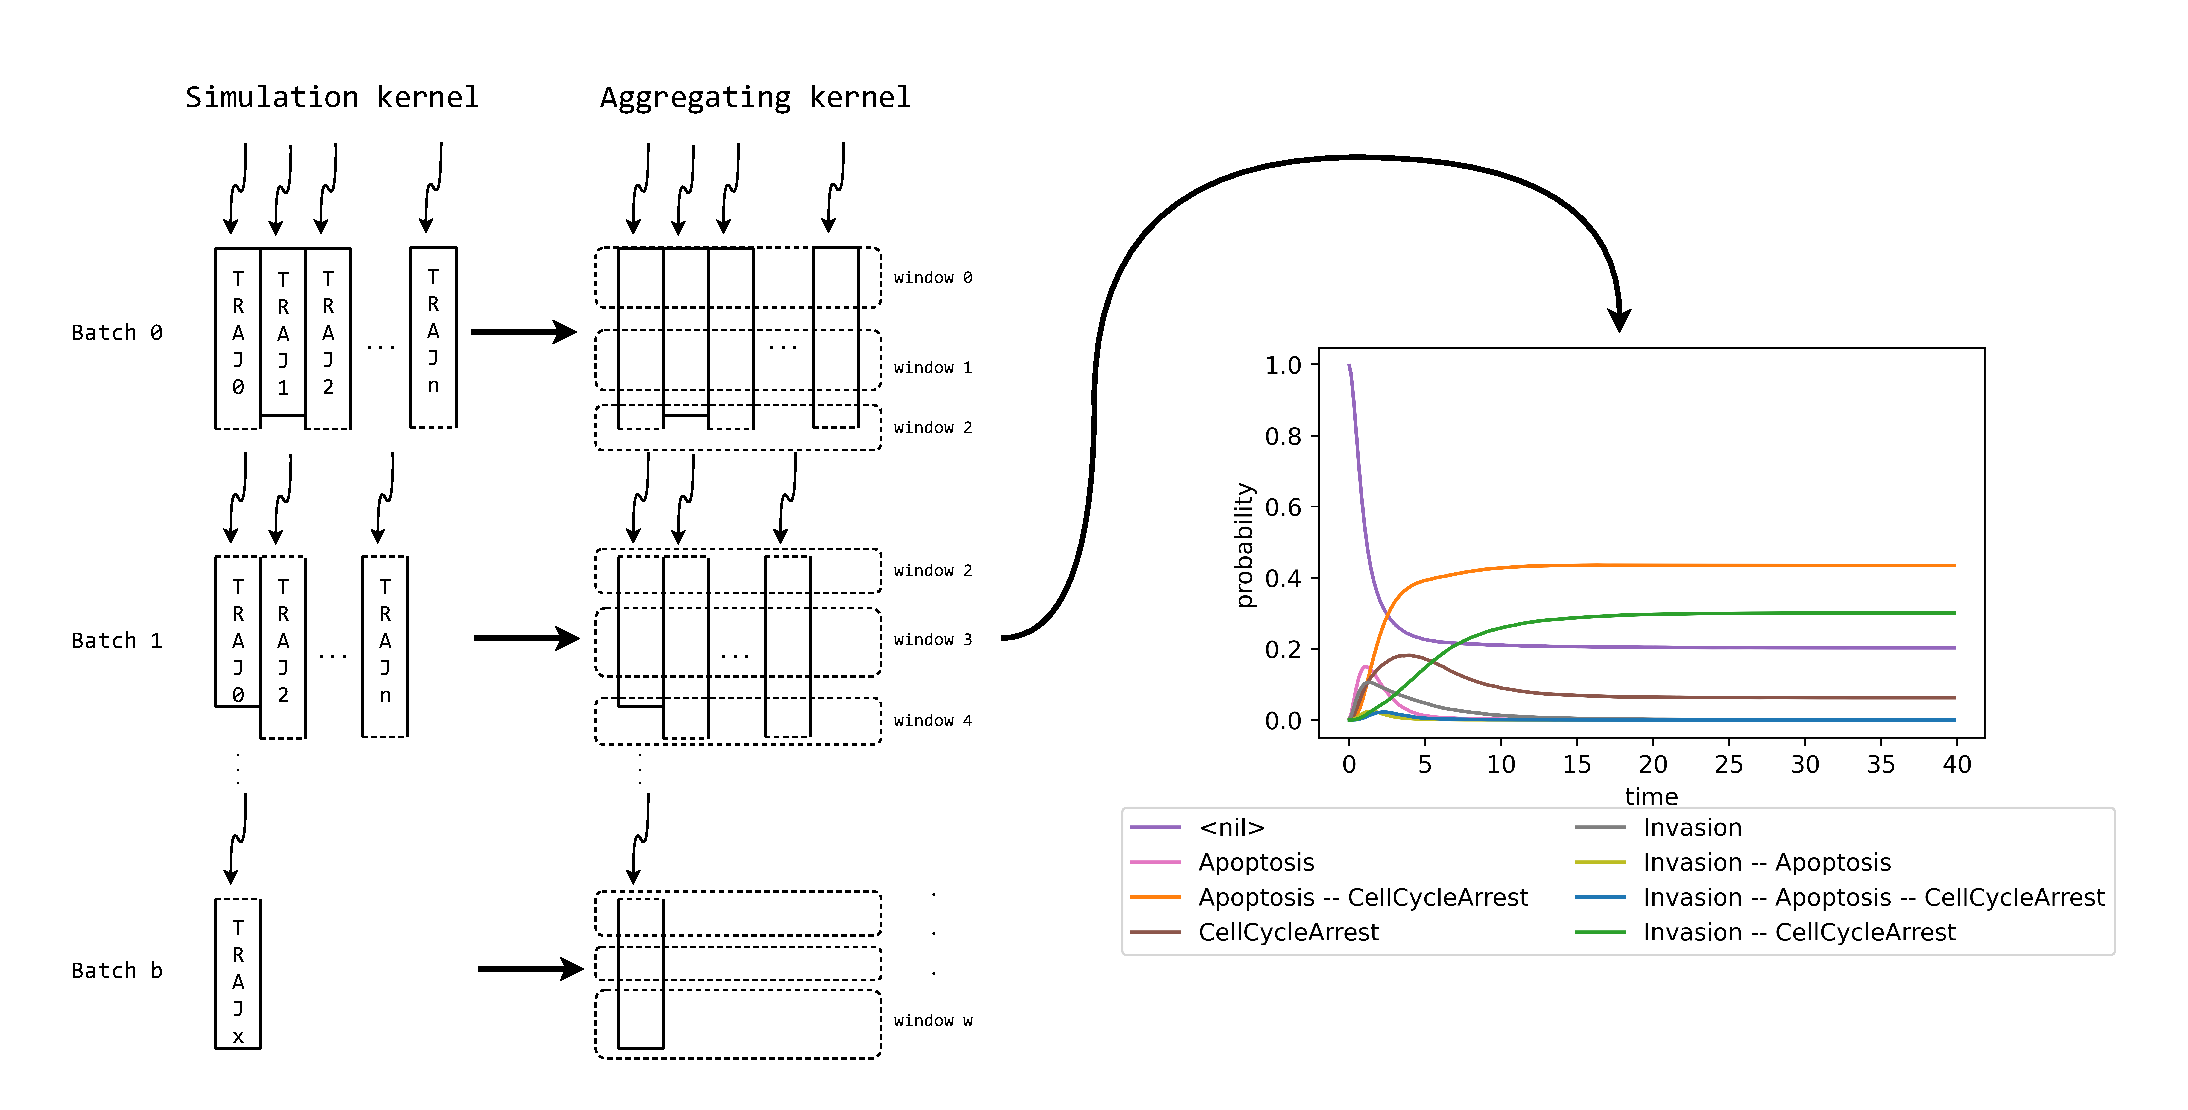
\includegraphics[width=\textwidth]{img/mabossg-kernels.pdf}
    \caption{The MaBoSS projection of simulated trajectories averaged over a specific time window.}
    \label{fig:maboss}
\end{figure}

\subsubsection{GPU acceleration challenges}

Although the parallelization of MaBoSS may seem straightforward, it includes challenges that can significantly affect the overall performance. The main issue is the traversal of the binary expression tree to evaluate the Boolean formulae requred to sample transition probabilities. Generally, traversing irregular data structures causes conditional branching and creates an irregular data access pattern (refers to \nameref{sec:divergence} and \nameref{sec:coalescing} in Section~\ref{sec:gpu_optim}). A combination of these issues may leave GPU heavily underutilized, gaining very little to no performance improvement over a well-parallelized CPU code.


In our work, we used the \emph{CUDA NVRTC}~\cite{nvrtc-online} runtime compilation library to compile the formulas on the fly. It has the benefit of encoding the formulas into a native binary code, removing the necessity to fetch the data from the memory each time the formula is evaluated. Apart from that, the compiler can run a set of optimizations on the code, further improving the performance. Consequently, the runtime compilation comes at the cost of an additional runtime. Thankfully, our benchmarking showed that the compilation time amortizes well for simulations with reasonably big inputs.

\subsubsection{Results}

The final implementation of the MaBoSS simulation achieved a speedup of $100-300\times$ on real-world datasets over the parallel CPU version. Moreover, we created a synthetic test suite to stress the scalability of the implementation, which showed that the GPU implementation can simulate models with thousands of nodes and billions of trajectories in minutes. These results suggest that the consumer laptop equipped with a GPU can simulate models that were previously restricted to high-end computers. Furthermore, the double and triple mutant analysis no longer belongs just to the domain of supercomputers but could become feasible on data center-grade GPUs. Overall, we believe that the GPU acceleration of the MaBoSS simulation can significantly improve the analysis of Boolean networks and enable researchers to explore complex models while conveniently using their personal computers.

\section{Summary}

This chapter presented the work of implementing four scientific algorithms in the HPC domain. Overall, the results have shown that employing GPUs to solve scientific problems can help researchers push the boundaries of the size, scale, and complexity of analyzed data while leveraging the computational power of their GPU-equipped personal computers or laptops.

Further summarizing the optimization used, it comes as no surprise that the most important aspect to consider when designing an optimized implementation is memory. Memory complexity, memory access patterns, memory hierarchies, and data caching repeatedly occurred in our implementation designs and have contributed the most to performance improvements.

Therefore, in the second chapter of this thesis we present novel methods for streamlining memory-related optimizations, which we collected during our optimization efforts and found them to be effective in aiding HPC programmers in writing optimized CPU or GPU code from scratch.


\chapter{Streamlining the development of parallel algorithms using Noarr}

% - many scientific algorithms are centered around a master data structure
%   - examples (matmul, transposition, physicell, ...)
% - the optimal run of these algorithms require an efficient memory traversal over the master data structure (both memory layout and traversal order) (both parallel and serial)
% - the domain experts usually can guess the optimal / close to optimal layout and traversal order
% - however, some optimizations require complex traversals that are very complex and error-prone to implement (tiling, levenstein, ...)
% - moreover, some traversting constants require tuning for different hardware (atlas)
% - other example is of a non expert who wants to speed up code by optimizing traversal - examples?
%   - there exist some dsls that can help with this
% - making this all by hand is very error-prone and time-consuming, unmantainable

% others do it too: cute, Kokos

% paper 1:
% - layout definition
% - allocation decoupling
% - layout agnostic
% - CUDA compatible
% - constants expressions
% - no overhead

% paper 2:
% - traversal definition / agnosticism
% - parallelism

Commonly, the core computation of scientific algorithms is centered around a master data structure. The examples include a matrix composed of cell features in an agent-based simulator~\cite{ghaffarizadeh2018physicell}, a grid of substrates in a diffusion solver~\cite{ghaffarizadeh2016biofvm}, a transition rates graph for Markov processes~\cite{koltai2020exact}, etc. In the vast majority of these algorithms, the location of the most performance-critical parts lies in a nested loop over these data structures.

Possibly due to the lack of hardware expertise, usually there is no special attention paid to the memory performance when such loops are written by the domain experts~\cite{clauss2000automatic}. As a result, the programs show poor data locality, spending most of the CPU cycles waiting for the memory pipeline to deliver the data. 

A plethora of research works confirm that changing the way how data is laid in memory or modifying the nested loops can result in a significant performance improvement~\cite{gong2018empirical,stengel2015quantifying,serpa2019memory}. Such optimizations may include decreasing the number of cache misses by grouping the operation on the same data together, employing prefetching by streamlining the memory access pattern, or utilizing the vector instructions by aligning the data in memory.

Arguably, given a nested loop to optimize, the expert in the performance optimization domain can pinpoint the biggest bottlenecks w.r.t. memory and propose close to optimal modifications with great probability. The most common modifications would include reordering the loops for the most possible serial access pattern and dividing the loops into tiles or strides to employ cache hierarchies~\cite{wolf1991data}. The problematic activity here, which takes the most programmers time, is putting these modifications into code. For example, let us have a nested loop of depth 3 with control variables \texttt{i, j, k} and bounds \texttt{I, J, K}. A simple tiling modification of the loop adds complexity in loop depth, variable count and index computation: 
\begin{minted}[fontsize=\footnotesize,breaklines]{c++}
for (i1 = 0; i1 < I / tile_I; i1++)
  for (j1 = 0; j1 < J / tile_J; j1++)
    for (k1 = 0; k1 < K / tile_K; k1++)
      for (i2 = 0; i2 < tile_I; i2++)
        for (j2 = 0; j2 < tile_J; j2++)
          for (k2 = 0; k2 < tile_K; k2++)
          // i=i1*tile_I+i2; j=j1*tile_J+j2; k=k1*tile_K+k2;
\end{minted}
Omitting corner cases, the code is already verbose and rather error-prone. Naturally, the complexity of the code grows with the complexity of the optimization.

Thankfully, many tools have been developed to alleviate this issue. Some provide automatic optimizations built within a compiler~\cite{trifunovic2010graphite,grosser2012polly}, some extend a compiler with pragma-like annotations to guide the optimization process~\cite{donadio2005language,yi2007poet,chen2008chill,namjoshi2016loopy} and others include ad-hoc solutions for a specific family of algorithms~\cite{9485033,AFANASYEV2021100707}. However, very little attention has been paid to aiding HPC programmers in writing the optimized code from scratch by providing them with a clean and maintainable way to express complex loop traversal and memory layout fit for their specific problem.

To alleviate and streamline the mundane programming tasks repeatedly encountered during our work on optimizing scientific algorithms, we focused our work on developing a C++ library \emph{Noarr}. The main benefit of the library is that it allows to expressively and extensively define memory layouts of regular $n$-dimensional arrays and provides loop transformation primitives for their optimal traversal. It empowers HPC experts to swiftly develop their optimizations as a clean, error-prone code open to autotuning and parallelism while staying within the borders of the C++ standard without adding any dependency on the final software product (which is an advantage for the deployment in a scientific community).

% Arguably, the biggest requirement for the optimal performance of these algorithms is such traversal over the master data structure that generates memory accesses in the most hardware-efficient way. This can either mean: the least number of cache misses, the best utilization of the memory hierarchy, loop unrolling, automatized vectorization. To have a brief perspective on the importance, a simple matrix transposition runs 50x faster when traverzing data in the right order.  

% Critically, the expert int the performance optimization domain can usually guess the optimal or close to optimal traversal. In a big majority of cases, the proper cache utilization is just a question of iterating the loops in the right order and data tiling. The issue, which takes the most programmers time and is the most error-prone, is putting these traverals into code. A simple example of writing a tiling loop of 3D grid already results in an index hell.

% Furthermore, some optimizations require tuning of their parameters to be most efficient on a given hardware. For memory optimizations, such tunable parameters would be for example a size of a tile to fit given cache, or loop unrolling factor to sattisty the width of vector memory/compute instructions. Carrying out these tasks not in an automatized way is unmantainable and time-consuming. There are whole projects targeting automatic optimizations of specific algorithms, such as atlas for matrix multiplcation, FFTW for FFT, SPIRAL for signal processing. cuTLASS for CUDA matrix multiplication

% To alleviate and streamline these mundane programming tasks, which we encountered during our work on optimizing scientific algorithms multiple times, we focused our work here and developed a pure C++ library Noarr. Naturally, there are other libraries that aim to solve the same problem, the added value of noarr is:
% \begin{itemize}
%   \item a pure c++ approach without any need for DLS or precompilers. It empowers HPC experts to swiftly code their optimizations error-prone without adding any dependency on the final product. Which is usually paid huge attention to in a scientific community.
%   \item allows for simple tuning of the traversal constants for different hardware
%   \item CUDA compatible
%   \item support for parallelization of the traversal
%   \item %take sth from cgo paper
% \end{itemize}


\section{Memory Layouts}

% - example of layout definition

% - example of traversal
% - how hard to define traversal by hand

% The main goal of noarr is to epressively and extensively define memory layouts and their traversals. There exists 

% definition of layout
% definition of traversal
% they are isomorphic, but layout can be stronger than traversal eg thanks to vector instructions
% there are not many libraries that allow to easily define custom layout.
% there are some, which do just a specific use cases, such as Kokkos (which is a big library and is specialized just on a set of specific use cases) GridTools similarly
% but recently, in parallel with our research, bigger players started to realize the importance of memory layout. ndspan in c++ standard and cute in cuda. ndspan is a good start, but noarr is much more extensible. cute was developed for Atlas, but it is not as general as noarr.
% noarr defines layout by composing atom protostructs
% column major, row major example in double for loop
% perhaps example of transformation c->r
% we require traversal to do it effectively
% for traversals, there are way more other tools that do the same. some of them do it automatically, polly. many of them are, however, annotation based, requiring custom compiler to precompile the code. or compiler pragmas. They target a different audience. similar comparison is openMP vs tbb. https://link.springer.com/content/pdf/10.1007/978-3-642-03869-3_62.pdf While TBB appears to be less appropriate for parallelizing existing implementations, it fosters a good programming style and higher abstraction level for newly developed parallel programs.
% show noarr traverse - some split tile example ... perhaps physicell

Generally, the way how data is laid in memory, a \emph{memory layout}, can be portrayed as a projection of its index space to a linear memory space. If we limit ourselves to a general (non-ragged) $n$-dimensional array, we can define memory layout mathematically as follows:

\begin{defn}[Memory Layout]
  Suppose a regular $n$-dimensional array $A$ with dimension lengths $d_1, \dots, d_n$ and an index space $\mathcal{I} = \{0,\dots,d_1 - 1\}\times \dots \times \{0,\dots,d_n - 1\}$. We define a \emph{memory layout} $\mathbb{L}$ of $A$ as a bijection $\mathbb{L}: \mathcal{I} \to \{0,\dots, \prod_{i}d_i - 1\}$. 
\end{defn}

Perhaps the most common memory layouts are row-major and column-major of a matrix. Their respective bijections can be generated by indexing functions $L_{\text{row}}(i,j) = i \cdot d_2 + j$ and $L_{\text{col}}(i,j) = j \cdot d_1 + i$ and these functions would be carried to source code with slight modifications. 

As alluded to in the motivation, common layouts used to optimize memory accesses require a complex code. A tiled matrix layout, the layout paramount for some algorithms to optimally use cache hierarchies, already requires a verbose indexing function. Helping ourselves with adding two intra-tile dimensions, the indexing function would look as follows:
$$L_{\text{tiled}}(i,j,k,l) = (((i \cdot d_2 + j) \cdot d_3) + k) \cdot d_4 + l$$
Arguably, adding another tile dimension (to utilize multiple levels of cache) or swapping intra-tile layout to column-major form becomes less and less trivial. Moreover, considering the indexing functions are written ad-hoc, the layouts are tough subjects to change since a layout change requires a thoughtful and error-prone rewrite of all index function occurrences. On top of that, a complex indexing function is far from self-describing, making it hard, even close to impossible, to guess the layout intentions.

\subsection{Background}

The importance of these issues has been recognized by the HPC community, especially by the authors of HPC programming frameworks. Perhaps the oldest example is Kokkos~\cite{CARTEREDWARDS20143202}, a platform-agnostic programming model that defined a memory layout as a \emph{first-class object}. The layout is defined as a vector of dynamic dimension lengths; the dimensions are laid out in memory from left to right (the leftmost dimension being laid in the memory continuously with a stride of 1, also called Fortran-style), from right to left (perhaps the most used one, C-style) or generally by a custom vector of strides. Such a simple approach covers a wide range of HPC use cases and has been adopted by other frameworks, such as GridTools~\cite{AFANASYEV2021100707}. An example of defining a layout with $3$ dimensions of lengths $3$, $3$ and $4$ and their respective strides $1$, $5$ and $20$ in Kokkos is as follows:

\begin{minted}[fontsize=\footnotesize,breaklines,frame=leftline]{c++}
  // Some storage
  int* ptr = new int[80];
  // A layout object with pairs of size and stride
  Kokkos::LayoutStride layout(3, 1, 3, 5, 4, 20);
  // A view from the pointer and the layout
  Kokkos::View<int***> w(ptr, layout);
  int elem = w(0, 0, 0);
\end{minted}


Recently, much bigger communities have started to invest time in designing an extensible way of defining layouts. C++ has standardized \emph{mdspan} in C++23. It takes a finer approach, allowing to define layout dimensions using a more complex extent structure. Such a structure enables defining some dimension lengths as static (known at compile time) and mix them with some dynamic (known at runtime). With such information during compile-time, a compiler can employ optimizations such as constant folding, loop unrolling, or automatized vectorization. Similarly, as with a vector of strides in Kokkos, it defines a \texttt{LayoutPolicy}, responsible for converting dimensions to underlying 1D memory. 

\begin{minted}[fontsize=\footnotesize,breaklines,frame=leftline]{c++}
  // Some storage
  int* ptr = new int[80];
  // An extent structure, the first two dims are static 
  std::extents<3, 3, std::dynamic_extent> ext(4);
  // mdspan object with a pointer, extents and Fortran-style layout policy
  std::mdspan<int, decltype(ext), std::layout_left> s(ptr, ext);
  int elem = s[0, 0, 0];
\end{minted}

Nvidia has recently introduced \emph{CuTe}, a collection of C++ CUDA template abstractions for defining and operating on hierarchically multidimensional layouts of threads and data~\cite{cute-online}. It follows similar principles as mdspan: it defines \emph{shape}, \emph{stride} and \emph{tensor} as alternatives to Extents, LayoutPolicy and mdspan. The same example as above written using CuTe lists as follows:

\begin{minted}[fontsize=\footnotesize,breaklines,frame=leftline]{c++}
  // Some storage
  int* ptr = new int[80];
  // A layout as a pair of shape and stride
  Layout l = make_layout(
    make_shape(Int<3>(), Int<3>(), 4),
    make_stride(Int<1>(), Int<3>(), Int<9>())
  );
  // A tensor object with a pointer and a layout
  Tensor t = make_tensor(ptr, l);
  int elem = t(0, 0, 0);
\end{minted}

Shapes and strides can be nested, creating a hierarchy of coordinates. Also, every layout (even a nested one) can be indexed with 1D coordinates, iterating the index space in a colexicografix order. This allows for a natural indexation of complicated layouts; e.g., a tiled matrix 4D layout can be indexed using standard 2D coordinates, hiding the complexity of the layout. 
Apart from that, CuTe also takes a formal approach, creating a \emph{layout algebra}. It defines a set of operations over layouts, such as concatenation, composition, tiling, etc. These operations are used to build more complex layouts from simpler ones.

% CuTe - much more formal approach - defines a layout algebra 
% more complex layout able to "hide dimensions"
% more complex stride, which does not have to 

% If you're familiar with the C++23 feature mdspan, this is an important difference between mdspan layout mappings and CuTe Layouts. In CuTe, Layout is a first class citizen, is natively hierarchical to naturally represent functions beyond row-major and column-major, and can similarly be indexed with a hierarchy of coordinates. (mdspan layout mappings can represent hierarchical functions as well, but this requires defining a custom layout.) Input coordinates for an mdspan must have the same shape as the mdspan; a multidimensional mdspan does not accept 1-D coordinates.

% CuTe provides an "algebra of Layouts" to support combining layouts in different ways. This algebra includes operations such as

% Layout functional composition,
% a notion of Layout "product" to reproduce one layout according to another, and
% a notion of Layout "divide" to split one layout according to another.
% Common utilities for building complicated layouts from simpler ones depend on the Layout product. Common utilities for partitioning layouts (of data, for example) across other layouts (of threads, for example) depend on the Layout divide. All of these utilities rely on the functional composition of Layouts.

% In this section, we'll build up the tools of the Layout algebra and explain some of these core operations in detail.

% The developers familiar with this issue by encapsulating the memory layout into a complete object representing a data structure. Kokkos, platform-agnostic programming model, provides a simple syntax to define a list of static or dynamic dimensions of a multi-dimensional regular array and allows user to specify if the dimensions should be layed in memory from left to right (C-style), from right to left (Fortran-style) or in a custom stride.
% GridTools provides a similar functionality, but it is more focused on the stencil computations and allows to select back-ends (GPU, multicore-CPU, \dots) according to which the most suitable layout will be selected. However, the memory layout is a very general concept and it is impossible to cover all the use-cases.

% The mentioned works are mainly focused on a generalized optimization of a specific set of algorithms. They implement ways to efficiently parallelize problems, distribute and aggregate data. Still, they discovered that memory layout is integral part of the optimization process. Hence, they integrated some freedom of layout selection as a part of their libraries.

% Standalone layouting stuff:
% In parallel with our research, other works have been done in this area. C++ standard introduces mdspan, which will provide basic layouting functionality in standard library as soon as C++23 with more coming C++26. NVIDIA also realised the importance of extensive layouts and introduced CuTe library with a simmilar layouting algebra.
% %https://arxiv.org/html/2312.11918v1/#S3

\subsection{Noarr Layouts}

Noarr aims to enhance the expressiveness, extendibility, and maintainability of the code. The main points which distinguish Noarr from other libraries are:

\begin{itemize}
  \item \emph{Named dimensions} --- the dimensions are not defined just by an order of shape or stride vectors, but they are named. This allows to query a dimension regardless of its global index.
  \item \emph{Proto-structures} --- a set of building blocks is provided to allow to easily define complex layouts by their various composition.
\end{itemize}

Let us give an example of a row-major matrix memory layout using noarr. Considering \mintinline{c++}{'i'} as a row dimension and \mintinline{c++}{'j'} as a column dimension, the layout can be defined as follows:

\begin{minted}[fontsize=\footnotesize,breaklines,frame=leftline]{c++}
  // Some storage
  int* ptr = new int[80];
  // A row-major matrix layout
  auto row_l = scalar<int>() ^ vector<'j', 'i'>(lit<3>, 4);
  // A bag object with a pointer and a layout
  bag b = make_bag(row_l, ptr);
  int elem = b.at<'i', 'j'>(0, 0);
\end{minted}

Although Noarr predates mdspan and CuTe, it shares many similarities: the separation of layout and underlying memory and the ability to define static and dynamic-sized dimensions. Perhaps the biggest difference is the absence of a stride vector. In Noarr, the strides are computed automatically according to the order of the named dimensions. The matrix layout above can be changed to column-major by a simple named dimensions swap:
\begin{minted}[]{c++}
auto col_l = scalar<int>() ^ vector<'i', 'j'>(4, lit<3>);
\end{minted}
The order in which the dimensions are defined signals the way how they are laid in memory, which is in the left-to-right fashion. The meaning of the dimension names is important here, as it determines the \emph{logical order}. The order in the definition then defines the \emph{physical order}. For example, let us have a cube layout, denoting its height, width and depth as \mintinline{c++}{'i'}, \mintinline{c++}{'j'} and \mintinline{c++}{'k'} respectively. A C-style cube layout could be defined using \mintinline{c++}{vector<'k', 'j', 'i'>()} proto-structure. A custom layout (neither Fortran- neither C-style) can be simply written as \mintinline{c++}{vector<'j', 'k', 'i'>()}. Using this logical-physical distinction, all of the vastly used stride vectors can be simulated by permuting the dimensions order.

The other aspect of Noarr is the way how the layout is defined --- as a composition of building blocks, the protostructures. We already mentioned \texttt{row\_l}, which is a composition of \mintinline{c++}{scalar<int>} and \mintinline{c++}{vector<'j', 'i'>}, which, when composed, represents a vector (\mintinline{c++}{'i'}) of vectors (\mintinline{c++}{'j'}) of integer scalars (\mintinline{c++}{int}) --- an integer matrix. The left-to-right reading of the layout definition allows for easy extension of existing layout. See examples of more complex layouts in Listing~\ref{lst:lll}.

\begin{listing}
  \begin{minted}[fontsize=\footnotesize,breaklines]{c++}
  // A layout for a batch of row-major matrices
  // and offset to the 1st row of the 2nd matrix
  auto batched_l = row_l ^ vector<'b'>(10);
  size_t o1 = batched_l | offset<'i', 'j', 'b'>(1, 0, 2);
  // A tiled matrix layout (both row-major and col-major, 
  // where 'k' and 'l' denote tile rows and columns)
  auto tiled_rr_l = row_l ^ vector<'l', 'k'>(5, 10);
  auto tiled_rc_l = row_l ^ vector<'k', 'l'>(10, 5);
  // A sublayout composed of the 3rd row tiles 
  auto tiled_3rd_l = tiled_rc_l ^ fix<'k'>(3);
  // A tiled matrix layout indexable using 2 coordinates
  auto tiled_2d_l = tiled_rr_l ^ merge_blocks<'i', 'k', 'I'>() ^ merge_blocks<'j', 'l', 'J'>();
  \end{minted}
  \caption{Examples of layout compositions in Noarr.}
  \label{lst:lll}
\end{listing}

These protostructures allow for expressing complex layouts in a readable and error-prone way. Their extensibility in composition and separation from the underlying memory also allows for plug-in layouts, which can be easily reused in different parts of the code.


% Noarr puts the biggest emphasis on expressiveness, perforamnce and extensibility of memory layouts. It is a standalone C++ header-only library based on template metaprogramming and is based on these principles:
% \begin{itemize}
%   \item \emph{named dimensions} The dimensions are not defined just by an order of some numbers, but they are named. This allows to query info of a dimension regardles its global index.
%   \item \emph{trivial layouts} A set of trivial layout transformers is provided to allow to easily define complex layouts by composition of simple transformations.
% \end{itemize}

% Noarr borrows trivial tranformations from a well-known set of loop transformation, but extends it with some more. These are dimension reordering, 
% strip mining, fusion, fission, but also a z-curve

% Let us give an example of row-major matrix memory layout using noarr. Considering \mintinline{c++}{'i'} as a row dimension and \mintinline{c++}{'j'} as a column dimension, the layout can be defined as follows:
% \begin{minted}[breaklines]{c++}
% auto row_major = scalar<float>() ^ sized_vector<'j'>(n) ^ sized_vector<'i'>(m);
% \end{minted}
% The layout reads from left to right, signaling the innermost dimension first. 
% It is apparent, that \mintinline{c++}{row_major} object represents only a layout, and to access the data, a memory pointer has to be provided:
% \begin{minted}[breaklines]{c++}
% float* data = new float[n * m];
% float element = row_major | get_at<'i', 'j'>(data, 0, 0);
% \end{minted}
% To define a column-major layout, preserving the semantics of the dimension name, the layout can be defined as follows:
% \begin{minted}[breaklines]{c++}
% auto col_major = scalar<float>() ^ sized_vector<'i'>(m) ^ sized_vector<'j'>(n);
% \end{minted}
% The layout can be modified even more by introducing multiple dimensions. For example, to define a tiled layout, we add two more dimensions for the tiles:
% \begin{minted}[breaklines]{c++}
% auto tiled = scalar<float>() ^ sized_vector<'l'>(tile_n) ^ sized_vector<'k'>(tile_m) ^ sized_vector<'j'>(n / tile_n) ^ sized_vector<'i'>(m / tile_m);
% \end{minted}
% Here shows the power of named dimensions. Physically (in memory), \mintinline{c++}{'l'} and \mintinline{c++}{'k'} dimensions are innermost, representing column and row of a tile respetively. Dimensions \mintinline{c++}{'j'} and \mintinline{c++}{'i'} are outermost, representing column and row of a matrix, whose elements are whole tiles. With such semantics, tiles are both among themselves and within in row-major format. Unsurprisingly, the inter-tile layout can be changed to column-major by a simple rewrite: 
% \begin{minted}[breaklines]{c++}
%   auto tiled = scalar<float>() ^ sized_vector<'k'>(tile_m) ^ sized_vector<'l'>(tile_n) ^ sized_vector<'j'>(n / tile_n) ^ sized_vector<'i'>(m / tile_m);
% \end{minted}


\section{Layout Traversals}

Having specified how a data structure is laid in memory, the other possible point of optimization lies in the order how the data structure is iterated, its \emph{traversal}. In general, a traversal is usually written as a sequence of nested loops, which in turn generates a sequence of memory accesses. Imaging such ordering as a bijection $\mathbb{T}: \{0, \dots, \prod_{i}d_i - 1\} \to \mathcal{I}$, where $\mathcal{I}$ denotes an index space of a data structure and $d_0, \dots, d_{n-1}$ represent the boundaries of nested loop of depth $n$, the traversal shares many similarities with the memory layout. From the perspective of accesses, in many cases, the same sequence of accesses can be generated by either changing the layout ($\mathbb{L}$) or the nested loop ($\mathbb{T}$). Therefore, same as with a layout, modifying a traversal can improve data locality, both in time and space. Although modifying traversal is constrained by data dependencies, loop transformation is still a well-researched topic and complements the memory layout optimization~\cite{clauss2000automatic}.

\subsection{Background}

Quantitatively, \emph{loop transformation} is perhaps more researched topic than layout transformation. Neither aforementioned library provides ways to transform a traversal, but there are many other tools that do. Contemporary compilers employ sophisticated loop optimizers based on the polyhedral model, such as Graphite in GCC~\cite{trifunovic2010graphite} or Polly in LLVM~\cite{grosser2012polly}. However, these optimizers are limited by the lack of information specified by the user in the code.

For more user-guided approaches, there are annotation-based tools, such as Poet~\cite{yi2007poet}, Chill~\cite{chen2008chill} or Loopy~\cite{namjoshi2016loopy}. These tools allow to specify the traversal transformations by adding special comments or pragmas to the code. The transformations are then applied by a precompiler, which generates the optimized code. Perhaps the best representative of annotation-based frameworks is done by Kruse et al.~\cite{kruse2018user}. The authors have presented pragma-based user-directed loop transformations for the Clang compiler, which has been partly adopted by the OpenMP standard. The transformations include loop tiling:
\begin{minted}[fontsize=\footnotesize,breaklines,frame=leftline]{c++}
  // original code
  #pragma clang loop(i,j) tile sizes(4,8)
  for (int i = 0; i < n; i+=1)
    for (int j = 0; j < m; j+=1)
  // transformed code
  for (int i1 = 0; i1 < n; i1+=4)
    for (int j1 = 0; j1 < m; j1+=8)
      for (int i2 = i1; i2 < n && i2 < i1+4; i2+=1)
        for (int j2 = j2; j2 < m && j2 < j1+8; j2+=1)
\end{minted}
or loop reordering:
\begin{minted}[fontsize=\footnotesize,breaklines,frame=leftline]{c++}
  // original code
  #pragma clang loop(i,j) interchange permutation(j,i)
  for (int i = 0; i < n; i+=1)
    for (int j = 0; j < m; j+=1)
  // transformed code
  for (int j = 0; j < m; j+=1)
    for (int i = 0; i < n; i+=1)
\end{minted}
but also loop fusion, fission, reversal and others~\cite{mckinley1996improving}. 

These tools are straightforward to use, and their ability to combine them to form complex loop transformations makes them very expressive. A minor downsight is that they are typically closed to extensions and for majority of them, a precompiler with an extra preprocessing step, or a custom compiler extension is needed.

On the other hand, the target problems for annotation-based loop transformation tools are somehow limited. Naturally, the best use of them is made when there is already a baseline implementation, and the optimization is achieved just by adding a few lines on the top of the loop with the hottest performance spots. However, when developing an optimized solution from scratch and when the scale of the program passes a certain complexity threshold, optimizing just by annotations may become cumbersome. 

A good evidence of this fact are case studies which compared the effort of programming a parallel algorithm using OpenMP, also a pragma-based library, with pure C++ libraries, such as TBB. The studies generally confirm that ease of expressing parallelism in OpenMP is traded for a lower abstraction level and flexibility. Language-based approaches, such as TBB, can utilize object-oriented design for more control, fostering of good programming style and higher abstraction level for \emph{newly} developed parallel programs~\cite{kegel2009using,ajkunic2012comparison,refsnes2011comparison}.

\subsection{Noarr Traversals}

The similarities in memory layout and its traversal led to the development of \emph{Noarr Traversals}. It is based on the idea that each single loop, in some sequence of nested loops, can be interpreted as one (named) dimension in index space domain. Assuming perfectly nested loops, such traversal can be interpreted as a Noarr layout and be subjected to the same transformations as a memory layout.

Let us highlight this idea on an example of matrix multiplication, where a plain C++ implementation would look like this:

\begin{minted}[fontsize=\footnotesize,breaklines,frame=leftline]{c++}
  for (int i = 0; i < m; i++) 
    for (int j = 0; j < n; j++) 
      for (int k = 0; k < p; k++) 
        C[i][j] += A[i][k] * B[k][j];
\end{minted}
The nested loops follow the order of $3$ present dimensions: $i$, $j$ and $k$ denoting rows of $C$ and $A$, columns of $C$ and $B$, and rows of $A$ and columns of $B$ respectively. Smartly selecting the named dimensions of the layouts, the traversal can be rewritten using Noarr as follows:

\begin{minted}[fontsize=\footnotesize,breaklines,frame=leftline]{c++}
  auto A = make_bag(ptr_a, scalar<int> ^ vector<'k', 'i'>(K, I));
  auto B = make_bag(ptr_b, scalar<int> ^ vector<'j', 'k'>(J, K));
  auto C = make_bag(ptr_c, scalar<int> ^ vector<'j', 'i'>(J, I));
  
  traverser(A, B, C) | [=](auto state) {
    C[state] += A[state] * B[state];
  };
\end{minted}

The traverser extracts dimensions from the passed-in layouts and yields an index space corresponding to the cartesian product of the extracted dimensions (after removing duplicates). Thanks to the dimensions naming, the index space is equivalent to the layout with $3$ dimensions \mintinline{c++}{'i'}, \mintinline{c++}{'j'} and \mintinline{c++}{'k'}, iterable in the same way as in the plain example.

As a result, changing the traversal order is done the same way as modifying the layout --- by applying the proto-structures to the traverser. E.g., to reorder the loops to a more cache-friendly \mintinline{c++}{'i'}, \mintinline{c++}{'k'}, \mintinline{c++}{'j'} order, the traversal can be rewritten as follows:

\begin{minted}[fontsize=\footnotesize,breaklines,frame=leftline]{c++}
  traverser(A, B, C) ^ reorder<'i', 'k', 'j'>() | [=](auto state) {
    C[state] += A[state] * B[state];
  };
\end{minted}

Some transformations change the nesting level of the underlying loops, e.g., during a strip-mine transformation, where a loop is split into two nested loops by a blocking factor~\cite{mckinley1996improving}. Following the Noarr paradigm of named dimensions, a strip-mine is well defined by a proto-structure \mintinline[fontsize=\footnotesize]{c++}{into_blocks}, which accepts the first dimension as the input, which should be present in the layout, and two output dimension, which will be newly added to the composed layout. Since all loops are tracked by their names, the user has full control over the output of a transformation and can safely chain multiple transformations together. A tiled matrix multiplication can be expressed as follows:
\begin{minted}[fontsize=\footnotesize,breaklines,frame=leftline]{c++}
  // breaking dimension 'i' into two new dimensions 'I' and 'x'
  auto tiles = into_blocks<'i', 'I', 'x'>(noarr::lit<16>)
  ^ into_blocks<'j', 'J', 'y'>(noarr::lit<16>)
  ^ into_blocks<'k', 'K', 'z'>(noarr::lit<16>)
  // using the new dimensions
  ^ reorder<'I', 'J', 'K', 'x', 'y', 'z'>(); 

  traverser(A, B, C) ^ tiles | [=](auto state) {
    C[state] += A[state] * B[state];
  }; 
\end{minted}

With this arsenal of proto-structures, Noarr provides options to specify many complex layouts and traversals. Noarr layouts and traversal library has been already field-tested and integrated into our ongoing research and we can confirm that the combination of present primitives with strongly-typed dimension semantics can alleviate the burden of explicit coding and still be helpful for writing highly performant code. We expect that our solution will add a new expressive tool to a high-performance programming toolset, simplifying the research focusing on tunings of prewritten computational kernels and building complex optimized parallel algorithms from scratch.

% \section{Auto-tuning and parallelism}

% A common benefit of the aforementioned annotation-based loop transformers is the ability to automatically search the transformation space and find the most optimal traversal. This process of \emph{autotuning} is especially useful when the code is supposed to run on different hardware. As an example, the different cache sizes or vector registers widths can be easily adapted to by the autotuning process~\cite{frigo1998fftw,puschel2004spiral,whaley1998automatically}. 

% The modular template-based design of Noarr allows us to mimic the autotuning systems. It is achieved by defining a layout or a traversal as an argument of a performance-critical function. That way, a function is agnostic of the layout or traversal specified and, regardless the passed-in layout, it will result in the same operations, just in a different order. Such layout-agnostic (or traveral-agnostic) functions can be called repeatedly with different combinations of layout and traversal transformations. Listing~\ref{lst:agn} shows an example of a transformation-agnostic function written using Noarr, used to generate a performance heatmap of the benchmarked transformations (Figure~\ref{fig:heatmap_all}).

% \begin{listing}
%   \begin{minted}[fontsize=\footnotesize,breaklines]{c++}
%   template <class A_t, class B_t, class C_t, class Order_t>
%   void matmul(A_t& A, B_t& B, C_t& C, Order_t my_order) 
%   {
%       traverser(A, B, C) ^ my_order | [=](auto state) {
%           C[state] += A[state] * B[state];
%       };
%   }
%   \end{minted}
%   \caption{Layout- and traversal- agnostic matrix multiplication.}
%   \label{lst:agn}
% \end{listing}

% \begin{figure}
%   \centering
%   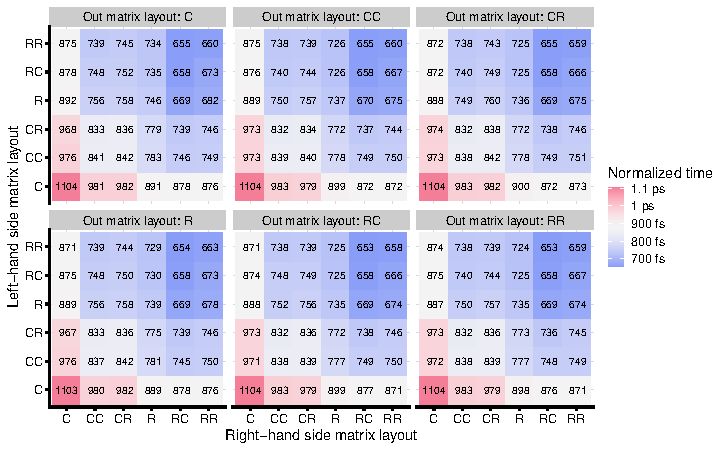
\includegraphics[width=0.8\textwidth]{img/heatmap_all}
%   \caption{Heatmap of the execution time of a matrix multiplication algorithm with different layout transformations. The optimal transformation is highlighted in blue.}
%   \label{fig:heatmap_all}
% \end{figure}

% Lastly, Noarr is compatible with parallelism. Noarr proto-structures are general enough to allow division of layouts and traversals into sublayouts and subtraversals for user-guided parallelism. Moreover, Noarr supports parallelization wrappers around TBB, OpenMP and CUDA, managing the division of the specified dimensions and assigning their traversal to parallel workers automatically.


% In the future, we plan to combine the proposed innovations
% with autotuning methods. The traversal-agnostic functions
% should provide an exciting starting point for the automated
% exploration of various traversal orderings. Furthermore, we
% are experimenting with using the layout-agnostic paradigm
% with the ultimate goal of designing a self-adaptive system
% that could change the layout of the data structures or even
% the order of loops at runtime.



% \subsection{layout agnostic code}

% Benefits of some annotation-based tools is the ability to automatically search transformation space and find the most optimal traversal. Such \emph{autotuning} is especially useful when the code is supposed to run on different hardware. The different cache sizes or vector registers widths can be easily adapted to by the autotuning process.

% As first-class objects, noarr layouts and traversals allow for \emph{layout-agnostic} and \emph{traversal-agnostic} code. A code, which contains the performance critical part, such as nested for loop of a scientific algorithm, can be encapsulated in a function, with traversal and layout extracted into function parameters:
% \begin{listing}
%   \begin{minted}[fontsize=\footnotesize,linenos,breaklines]{c++}
%   template <class A_t, class B_t, class C_t, class Order_t>
%   void matmul(A_t& A, B_t& B, C_t& C, Order_t my_order) 
%   {
%       traverser(A, B, C).order(my_order).for_each([&](auto Aidxs, auto Bidxs, auto Cidxs)
%       {
%           C.at(Cidxs) += A.at(Aidxs) * B.at(Bidxs);
%       });
%   }
%   \end{minted}
%   \caption{Traversal-agnostic matrix multiplication}
%   \label{lst:agn}
% \end{listing}

% The function can be called repeatedly with a different combination of layout and traversal transformations. Benchmarking the differently parametrized functions then shows the optimal transformations on a running hardware and highlights the most effective optimizations on a general hardware.

% % add figure heatmap_all


% The modular template-based design of this extension al-
% lows us to mimic the autotuning systems, which search the
% vast space of transformation, trying to find the most per-
% formant one for a specific computational function. In our
% approach, we may be able to express precisely that with
% so-called traversal-agnostic functions — the body of such
% functions does not change, although the traversal order does
% (see Listing 7).

% Our approach may promote less time spent in code compiling as we do not require to modify the source code when applying the different transformations. However, this is farfrom the scope of this paper.

% benefits of some of annotation based tools is the ability to autotune some layout parameters
% noarr layout agnostic abstraction allows just the same
% example of layout agnostic
% code can run irrespective the traversal used (assuming the traversal is correct)(isomorphic)
% find sth from cgo paper


% \section{parallelism}

% parallelism is a different kind of beast, it can alter the traversal
% considering algorithms with master data structures, the parallelism is usually a question of in which nested loop are we aiming to parallelize
% there can be caveats ofcourse, such as data dependencies, but they are usually easy to spot
% there can be caveats, such as different hierarchies of parallelsim (either be it simd on CPUs or more prevalent GPU) - so there is a need to divide in multiple levels
% noarr traversals are general enough to do this in a custom way
% nevetherless, we experimented with wrappers around tbb to provide proof of concept
% wrapper around cuda kernel launch which divides over 2 dims
% structure for cuda shared mem?
% examples




\chapwithtoc{Conclusion}

This thesis summarizes several efforts to improve the performance of complex algorithms with inefficient implementations from contemporary scientific domains, improving their practical usability by applying high-performance computing principles. In the two chapters, it outlines the motivations and results of six research contributions, presented in \cref{chap:contributions}.

The first four contributions detail the parallelization and optimization challenges of the scientific algorithms which we have worked on during our research. The results include GPU applications that use novel data structures, promote high scalability, and utilize complicated GPU optimization techniques. The presented implementations provide orders of magnitude speedups over the prior state-of-the-art, enabling domain scientists to finish their analyses in minutes instead of days, process more data with greater accuracy, interactively visualize the results, and explore previously unattainable problem variations. The methodology of the works can serve as a helpful support for other researchers in the domain of GPGPU computing.

The last two contributions present the use cases of the novel HPC library Noarr, specializing in expressing the layout and traversal of $n$-dimensional arrays, which are the most commonly used data structures in scientific computing. The novel approach of assigning names to the dimensions of the arrays and expressing the layout and traversal in a declarative way allows users to deploy memory-related optimizations in a more readable and maintainable manner while the library takes care of the complex indexing and loop transformations.

As implied throughout the thesis, the use of GPUs for general computing is becoming increasingly popular. Consequently, these devices improve in versatility with each addition of new core types, specialized high-throughput instructions, and new thread hierarchies. This creates unique and interesting opportunities for future research: The implementation of Mahalanobis Hierarchical Clustering can be directly extended with the use of tensor cores, which may provide an additional order of magnitude performance improvement thanks to their high compute bandwidth. Similarly, we plan to continue on $k$-NN development, which we have already started during the work on EmbedSOM, as we believe that increasing the caching capabilities by employing the new feature of distributed shared memory may improve the data throughput of such a highly memory-bound algorithm. To support the efforts, we plan to continue extending the Noarr library towards the auto-tuning direction, ultimately providing a machine learning-guided optimizer of the array layouts and traversals. We also plan to finish our work on biological simulations, especially BioFVM and PhysiCell, which has already served as a valuable case study for Noarr and has partly guided its development thanks to the presence of multiple complex high-dimensional arrays, which accelerated its usability.

Finally, we hope that the contributions of this thesis will help to develop software that performs well in spite of the impending technical challenges and progressive widening of the bandwidth-compute gap. We believe that the presented methodologies and contributions provide valuable insights that can serve as a foundation for further research in the field of GPGPU computing and HPC.

%%% Bibliography (literature used as a source)
%%%
%%% We employ bibTeX to construct the bibliography. It processes
%%% citations in the text (e.g., the \cite{...} macro) and looks up
%%% relevant entries in the bibliography.bib file.
%%%
%%% The \bibliographystyle command selects, which style will be used
%%% for references from the text. The argument in curly brackets is
%%% the name of the corresponding style file (*.bst). Both styles
%%% mentioned in this template are included in LaTeX distributions.

\bibliographystyle{plainnat}    %% Author (year)
% \bibliographystyle{unsrt}     %% [number]

\renewcommand{\bibname}{Bibliography}

%%% Generate the bibliography. Beware that if you cited no works,
%%% the empty list will be omitted completely.

\bibliography{bibliography}

%%% If case you prefer to write the bibliography manually (without bibTeX),
%%% you can use the following. Please follow the ISO 690 standard and
%%% citation conventions of your field of research.

% \begin{thebibliography}{99}
%
% \bibitem{lamport94}
%   {\sc Lamport,} Leslie.
%   \emph{\LaTeX: A Document Preparation System}.
%   2nd edition.
%   Massachusetts: Addison Wesley, 1994.
%   ISBN 0-201-52983-1.
%
% \end{thebibliography}


\chapwithtoc{List of publications}
\label{chap:publist}

The table below outlines the relative contributions of the authors in each publication, followed by a complete list of references. In the table, an empty circle indicates little to no contribution, a partially filled circle indicates partial to significant contribution, and a full circle signifies work done entirely or almost entirely by the author. Entries marked with an asterisk (*) have not yet successfully passed peer review at the time of submitting the thesis (June 2024). The underlined entries represent the main contributions of this thesis.

\subsubsection*{Relative contributions}
\begin{center}\sf\footnotesize
\begin{tabular}{cllcccc}
\toprule
Ref. & Channel& Year & Analysis & Impl. & Eval. & Writing \\
\midrule
(a) & \underline{Euro-Par} & 2021
    & \contF & \contF & \contF & \contP \\
(b) & \underline{ICA3PP} & 2022
    & \contP & \contN & \contP & \contP \\
(c) & arXiv & 2022 $\ast$
    & \contP & \contP & \contP & \contP \\
(d) & \underline{GPGPU}  & 2024
    & \contP & \contP & \contP & \contF \\
(e) & \underline{JPDC} & 2024 $\ast$
    & \contN & \contN & \contF & \contP \\
(f) & \underline{BMC Bioinfo.} & 2024
    & \contF & \contF & \contF & \contF \\
(g) & \underline{PMAM} & 2024
    & \contP & \contN & \contP & \contN \\
\bottomrule
\end{tabular}
\end{center}

\subsubsection*{Complete list of references}
\def\showpublication#1{\begin{refsection}\fullcite{#1}\end{refsection}}
\begin{enumerate}[(a),itemsep=0.2ex]
\item\showpublication{vsmelko2021gpu}
\item\showpublication{vsmelko2022astute}
\item\showpublication{vsmelko2022scalable}
\item\showpublication{10.1145/3649411.3649414}
\item\showpublication{jpdc-in-progress}
\item\showpublication{vsmelko2024maboss}
\item\showpublication{klepl2024pure}
\end{enumerate}



\openright
\end{document}
